\documentclass[main.tex]{subfiles}

\begin{document}

\subsection{Primo esercizio}

\begin{figure}[H]
\centering
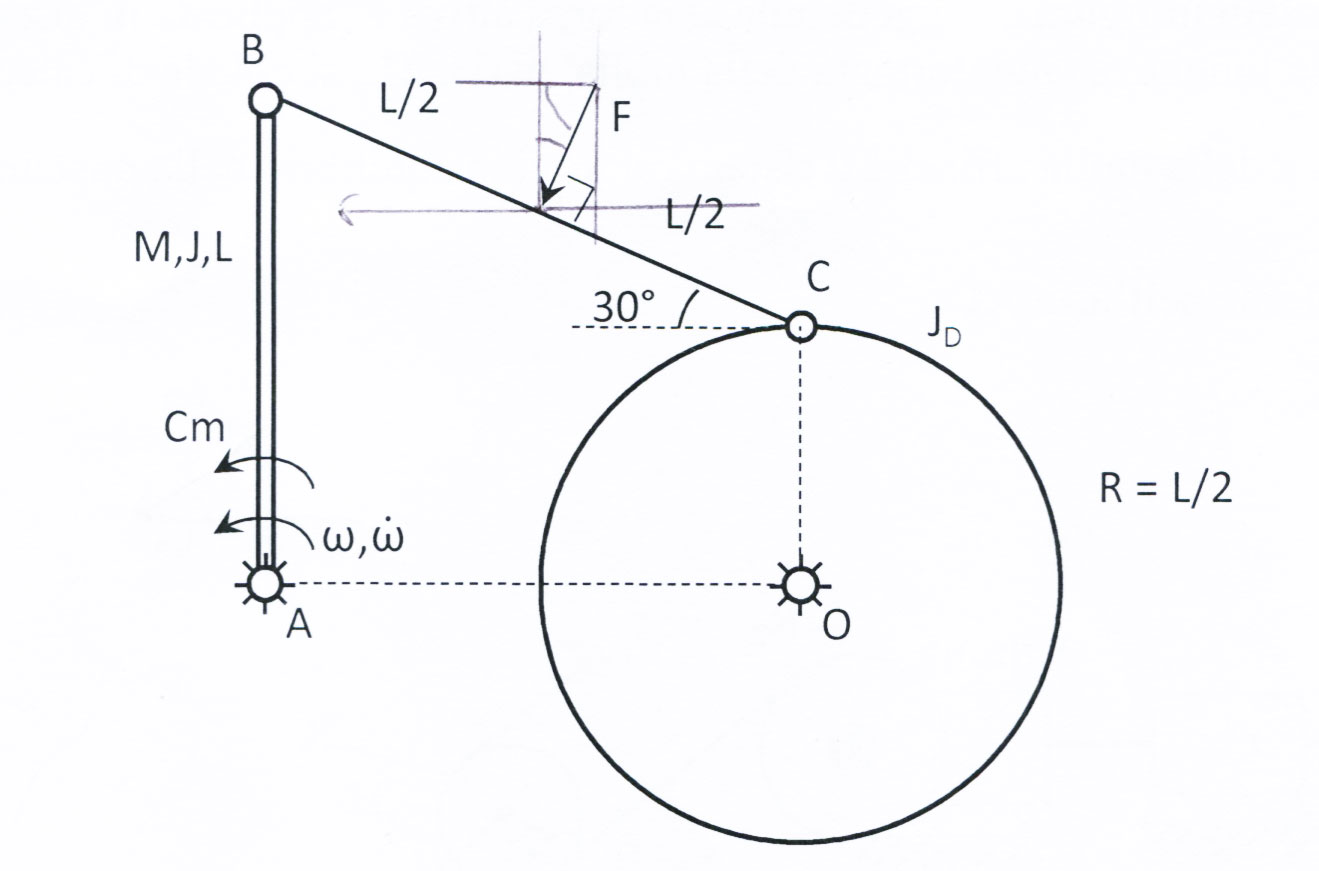
\includegraphics[width=0.75\textwidth]{2017-1109-1.jpg}
\end{figure}

\[
	L = 0.5\,m\quad
	M = 10\,Kg\quad
	J = 0.2\,kgm^2\quad
	J_D = 0.5\,kgm^2\quad
	F = 100\,N\quad
	\omega = 1\,rad/s\quad
	\dot{\omega} = 3\,rad/s^2
\]

Il sistema rappresentato in figura è posto nel piano verticale. L'asta omogenea \textbf{AB}, avente massa \textbf{M}, momento d'inerzia $J$ e lunghezza $L$, è incernierata a terra in \textbf{A}, mentre in \textbf{B} è incernierata ad un'altra asta \textbf{BC}, avente lunghezza $L$ e massa trascurabile.

L'asta \textbf{BC} è incernierata nel punto C ad un disco (avente momento d'inerzia $J_D$ e raggio $R = \dfrac{L}{2}$), a sua volta incernierato a terra nel proprio baricentro \textbf{O}. Come indicato in figura, sull'asta \textbf{AB} agisce una coppia $C_m$, mentre sul punto medio dell'asta \textbf{BC} agisce una forza $F$ nota e diretta come in figura.

Nota la geometria del sistema e assegnate la velocità e accelerazione angolare dell'asta \textbf{AB}, si chiede di calcolare:
\begin{enumerate}
\item La velocità e accelerazione angolare del disco.
\item La coppia $C_m$ necessaria per garantire la condizione di moto assegnata.
\end{enumerate}

\clearpage

\subsection{Risoluzione primo esercizio (non verificata)}

\subsubsection{Primo punto}

\paragraph{Equazione di chiusura}
Identifico come equazione di chiusura il quadrilatero $(A_B) + (B-C) = (A-0) + (O-C)$ ed assegno le seguenti variabili:

\[
	a = BA = 0.5\,m\quad
	b = BC = 0.5\,m\quad
	c = CO = 0.25\,m\quad
	d = AO = 0.5\cos\left( \dfrac{\pi}{6} \right ) = \dfrac{\sqrt{3}}{4}\,m
\]

Inoltre, definisco $\alpha$ l'angolo che descrive l'orientamento di AB, $\beta$ di BC e $\gamma$ di OC. I valori iniziali che questi angoli assumono sono i seguenti:

\[
	\alpha = \dfrac{\pi}{2}\,rad\quad
	\beta = -\dfrac{\pi}{6}\,rad\quad
	\gamma = \dfrac{\pi}{2}\,rad
\]

\paragraph{Spostamento}
\[
	ae^{i\alpha} + be^{i\beta} = d + ce^{i\gamma}
\]

\paragraph{Velocità}
\[
	a\dot{\alpha}e^{\left( \dfrac{\pi}{2} + \alpha \right )} + b\dot{\beta}e^{\left( \dfrac{\pi}{2} + \beta \right )} =  c\dot{\gamma}e^{\left( \dfrac{\pi}{2} + \gamma \right )}
\]

Separo in componenti cartesiane:

\[
\begin{cases}
	a\dot{\alpha}\cos\alpha + b\dot{\beta}\cos\beta = c\dot{\gamma}\cos\gamma\\
	-a\dot{\alpha}\sin\alpha - b\dot{\beta}\sin\beta = -c\dot{\gamma}\sin\gamma
\end{cases}
\]

È possibile semplificare il sistema notando che, nell'istante considerato, $\alpha = \gamma = \dfrac{\pi}{2}$:

\[
\begin{cases}
	b\dot{\beta}\cos\beta = 0\\
	-a\dot{\alpha} - b\dot{\beta}\sin\beta = -c\dot{\gamma}
\end{cases}
\]

Nella prima relazione, $b\neq0$ e $\cos\beta = \dfrac{\sqrt{2}}{2} \neq 0$, per cui $\dot{\beta} = 0\,rad/s$.

\[
\begin{cases}
	\dot{\beta} = 0\,rad/s\\
	\dot{\gamma} = \dfrac{a}{c}\dot{\alpha} = 2\,rad/s
\end{cases}
\]

\paragraph{Accelerazione}
\[
a\ddot{\alpha}e^{\left( \dfrac{\pi}{2} + \alpha \right )} - a\dot{\alpha}^2e^{i\alpha} + b\ddot{\beta}e^{\left( \dfrac{\pi}{2} + \beta \right )} - b\dot{\beta}^2e^{i\beta}=  c\ddot{\gamma}e^{\left( \dfrac{\pi}{2} + \gamma \right )}  - c\dot{\gamma}^2e^{i\gamma}
\]

Sostituisco $\dot{\beta}=0$ per semplificare l'espressione:

\[
a\ddot{\alpha}e^{\left( \dfrac{\pi}{2} + \alpha \right )} - a\dot{\alpha}^2e^{i\alpha} + b\ddot{\beta}e^{\left( \dfrac{\pi}{2} + \beta \right )}=  c\ddot{\gamma}e^{\left( \dfrac{\pi}{2} + \gamma \right )}  - c\dot{\gamma}^2e^{i\gamma}
\]

Separo in componenti cartesiane:

\[
\begin{cases}
a\ddot{\alpha}\cos\alpha - a\dot{\alpha}^2\sin\alpha + b\ddot{\beta}\cos\beta = c\ddot{\gamma}\cos\gamma - c\dot{\gamma}^2\sin\gamma\\
-a\ddot{\alpha}\sin\alpha - a\dot{\alpha}^2\cos\alpha - b\ddot{\beta}\sin\beta = -c\ddot{\gamma}\sin\gamma - c\dot{\gamma}^2\cos\gamma\\
\end{cases}
\]

È possibile nuovamente semplificare il sistema notando che, nell'istante considerato, $\alpha = \gamma = \dfrac{\pi}{2}$.

\[
\begin{cases}
- a\dot{\alpha}^2 + b\ddot{\beta}\cos\beta =  - c\dot{\gamma}^2\\
-a\ddot{\alpha} - b\ddot{\beta}\sin\beta = -c\ddot{\gamma}\\
\end{cases}
\Longrightarrow
\begin{cases}
\ddot{\beta} =  \dfrac{a\dot{\alpha}^2 - c\dot{\gamma}^2}{b\cos\beta} = -1.33\,rad/s^2\\
-a\ddot{\alpha} - (a\dot{\alpha}^2 - c\dot{\gamma}^2)\tan\beta = -c\ddot{\gamma}\\
\end{cases}
\]
\[
\begin{cases}
\ddot{\beta} =  \dfrac{a\dot{\alpha}^2 - c\dot{\gamma}^2}{b\cos\beta} = -1.33\,rad/s^2\\
\ddot{\gamma} = \dfrac{a\ddot{\alpha} + (a\dot{\alpha}^2 - c\dot{\gamma}^2)\tan\beta}{c} = 7.15\,rad/s^2\\
\end{cases}
\]

\subsubsection{Secondo punto}
Uso il bilancio delle potenze per calcolare la coppia.

\paragraph{Energia cinetica}

\[
E_c = \dfrac{1}{2}J\omega^2 + \dfrac{1}{2}J_D\dot{\gamma}^2 + \dfrac{1}{2}Mv_g^2
\]

Sostituisco con i legame $v_g = \omega \dfrac{L}{2} $.

\[
E_c = \dfrac{1}{2}J\omega^2 + \dfrac{1}{2}J_D\dot{\gamma}^2 + \dfrac{1}{2}M(\omega \dfrac{L}{2})^2
\]

Derivo l'espressione ed ottengo:

\[
\dfrac{E_c}{dt} = J\omega\dot{\omega} + J_D\dot{\gamma}\ddot{\gamma} + M\omega\dot{\omega}(\dfrac{L}{2})^2
\]

\paragraph{Potenza totale}

\[
\sum W_i = \vec{F}_g\bullet\vec{v}_{g_{AB}} + \vec{F}\bullet\vec{v}_{g_{BC}} + \vec{C}_m\bullet\dot{\omega}
\]

\begin{enumerate}
\item La forza di gravità $F_g$ forma un angolo di $\dfrac{\pi}{2}$ con la velocità $v_{g_{AB}}$, per cui non contribuisce alla potenza totale.
\item La forza $F$ forma un angolo di $\dfrac{\pi}{3}$ con la forza $v_{g_{BC}}$, che siccome $\dot{\beta} = 0$ la velocità del baricentro coincide con quella degli estremi.
\end{enumerate}

\[
\sum W_i = Fv_{g_{BC}}\cos\left ( \dfrac{\pi}{3} \right ) = \dfrac{1}{2}F\omega \dfrac{L}{2} = \dfrac{1}{4}F\omega L + C_m\omega
\]

\paragraph{Bilancio di potenze}

\[
	\dfrac{1}{4}F\omega L + C_m\omega = J\omega\dot{\omega} + J_D\dot{\gamma}\ddot{\gamma} + M\omega\dot{\omega}(\dfrac{L}{2})^2
\]

\[
	C_m = J\dot{\omega} + \dfrac{J_D\dot{\gamma}\ddot{\gamma}}{\omega} + M\dot{\omega}(\dfrac{L}{2})^2 - \dfrac{1}{4}F L = -2.875\,Nm
\]

\end{document}
